\documentclass%
%[handout]
{beamer}
% % % % % % % %
% % % % % % % %
% % % % % % % %
%IMPORTANT
%compiles with 
%pdflatex -shell-escape 
%IMPORTANT
% % % % % % % %
% % % % % % % %
% % % % % % % %
\mode<presentation>
{
\useinnertheme{rounded}
\useoutertheme{infolines}
\usecolortheme{orchid}
\usecolortheme{whale}
}

\usepackage[english]{babel}
\usepackage[latin1]{inputenc}
\usepackage[all,cmtip]{xy}
\usepackage{times}
\usepackage[T1]{fontenc}
\usepackage{../example-templates}
\usepackage{../pstricks-commands}

\usepackage{auto-pst-pdf}
\usepackage{pst-plot}
%\usepackage{pstricks-add} 

% Or whatever. Note that the encoding and the font should match. If T1
% does not look nice, try deleting the line with the fontenc.


\graphicspath{{../../modules/}}

\newtheoremstyle{partialproof}{3pt}{3pt}{}{}{}{.}{.5em}{}
\theoremstyle{partialproof} \newtheorem{partialproof}[theorem]{Proof.}
%\DeclareMathOperator{\diff}{d}
\setbeamertemplate{navigation symbols}{}

\includeonlylecture{1}

\newcommand{\lect}[3]{
  \date{#1}
  \lecture[#1]{#2}{#3}
}

\setbeamertemplate{footline}
{
  \leavevmode%
  \hbox{%
  \begin{beamercolorbox}[wd=.333333\paperwidth,ht=2.25ex,dp=1ex,center]{author in head/foot}%
    \usebeamerfont{author in head/foot}\insertshortauthor
  \end{beamercolorbox}%
  \begin{beamercolorbox}[wd=.333333\paperwidth,ht=2.25ex,dp=1ex,center]{title in head/foot}%
    \usebeamerfont{title in head/foot}\insertshorttitle
  \end{beamercolorbox}%
  \begin{beamercolorbox}[wd=.333333\paperwidth,ht=2.25ex,dp=1ex,center]{date in head/foot}%
    \usebeamerfont{date in head/foot}\insertshortdate{}
  \end{beamercolorbox}}%
  \vskip0pt%
}

% If you have a file called "university-logo-filename.xxx", where xxx
% is a graphic format that can be processed by latex or pdflatex,
% resp., then you can add a logo as follows:

%\pgfdeclareimage[height=0.8cm]{logo}{bluelogo}
%\logo{\pgfuseimage{logo}}
\renewcommand{\Arcsin}{\arcsin}
\renewcommand{\Arccos}{\arccos}
\renewcommand{\Arccot}{\text{arccot}}
\renewcommand{\Arctan}{\arctan}


\begin{document}

\AtBeginLecture{%

\title[\insertlecture]{FreeCalc}
\subtitle{\insertlecture}
\author[FreeCalc]{}
\institute[UMass Boston]{University of Massachusetts Boston}
\date{\insertshortlecture}
\begin{frame}
  \titlepage
\end{frame}
}%

% begin lecture
\lect{\today}{Sample}{1}

%% begin module arcsin-sin-ex1
\begin{frame}
\begin{example}
Find $\Arcsin (\sin 1.5)$.  
\begin{itemize}
\item<2->  \alert<2-3>{$\pi/2 \approx \uncover<3->{1.57.}$}
\item<4->  Therefore $-\pi/2 \leq 1.5\leq \pi/2$.  
\item<5->  Therefore $\Arcsin (\sin 1.5) = 1.5$.  
\end{itemize}
\end{example}
\end{frame}
% end module arcsin-sin-ex1

%% begin module arcsin-sin-ex2
\begin{frame}
\begin{example}
Find $\Arcsin (\sin 2)$.
\begin{itemize}
\item<2-> $2$ is not between $-\frac{\pi}{2}$ and $\frac{\pi}{2}$.
\item<3-> We need the angle \alertNoH{8,12}{$a$ between $-\frac{\pi}{2}$ and $\frac{\pi}{2}$} for which $\alertNoH{11}{ \alertNoH{4}{ \sin 2} =\alertNoH{7}{ \sin a}}$.
\end{itemize}
\uncover<9->{
\[
\begin{array}{rcl}
\alertNoH{9,10,13}{a} &\alertNoH{9,10,13}{=}& \fcAnswer{10}{ \alertNoH{13}{\pi - 2}.} \\
\uncover<11->{\text{Therefore }\quad \Arcsin(\alertNoH{11}{\sin 2}) &\alertNoH{0}{ =} & \alertNoH{12}{\Arcsin(\alertNoH{11}{\sin a})}} \\
\uncover<12->{&\alertNoH{0}{ =}& \worksheet{ \alertNoH{12,13}{ a} \uncover<13->{\alertNoH{13}{= \pi-2}.}}}
\end{array}
\]
}
\end{example}

\hfill
\psset{xunit=1.5cm, yunit=1.5cm}
\begin{pspicture}(-1.4,-1.4)(1.4,1.4)
\tiny
\fcAxesStandard{-1.2}{-1.2}{1.2}{1.2}
\parametricplot[linecolor=gray]{0}{360}{t cos t sin}%
\parametricplot[linecolor=brown]{-90}{90}{t cos t sin}%
\fcXTickWithLabel{1}{$1$}
\pstVerb{20 dict begin /pi 3.141592654 def /toDeg {180 mul pi div} def}%
\uncover<2->{%
\psline[arrows=->](0,0)(! 2 toDeg cos 1.3 mul 2 toDeg sin 1.3 mul)%
\parametricplot[linecolor=orange]{0}{2 toDeg}{t cos 0.35 mul t sin 0.35 mul}%
\rput[bl](0.24, 0.27){$2 $}
}%
\worksheet{%
\uncover<4->{\fcPerpendicular[linecolor=blue]{[2 toDeg cos 2 toDeg sin]}{[1 0]}{0.1}}%
\uncover<handout:0|4>{\psline[linecolor=blue, linewidth=2pt](! 2 toDeg cos 2 toDeg sin)(! 2 toDeg cos 0)}%
\uncover<5->{\parametricplot[linecolor=green]{2 toDeg}{180}{t cos 0.15 mul t sin 0.15 mul}%
\rput[br](-0.15, 0.15){$\fcAnswer{10}{\pi-2}$}%
}%
\uncover<handout:0|10>{%
\parametricplot[linewidth=2pt, linecolor=green]{2 toDeg}{180}{t cos 0.15 mul t sin 0.15 mul}%
\parametricplot[linewidth=2pt, linecolor=green]{0}{pi 2 sub toDeg}{t cos 0.15 mul t sin 0.15 mul}%
}%
\uncover<6->{%
\psline[linestyle=dotted](! 2 toDeg cos 2 toDeg sin)(! pi 2 sub toDeg cos pi 2 sub toDeg sin)%
}%
\uncover<7->{%
\fcPerpendicular[linecolor=blue]{[pi 2 sub toDeg cos pi 2 sub toDeg sin]}{[-1 0]}{0.1}%
\psline[arrows=->](0,0)(! pi 2 sub toDeg cos 1.3 mul pi 2 sub toDeg sin 1.3 mul)%
}%
\uncover<handout:0|7>{\psline[linecolor=blue, linewidth=2pt](! pi 2 sub toDeg cos pi 2 sub toDeg sin)(! pi 2 sub toDeg cos 0)}%
\uncover<8->{%
\parametricplot[linecolor=green]{0}{pi 2 sub toDeg}{t cos 0.15 mul t sin 0.15 mul}%
\rput[lb](0.15, 0.07){$\alertNoH{9,10}{a}$}%
}%
}%
\pstVerb{end}
\end{pspicture} \quad 
\psset{xunit=1.0cm,yunit=1.0cm}
\begin{pspicture}(-2.2,-1.9)(4.2,1.9)
\tiny
\pstVerb{20 dict begin /pi 3.141592654 def /toDeg {180 mul pi div} def}%
\psaxes[labels=none, Dx=1.570796327, Dy=1] {<->}(0,0)(-2,-1.8)(4,1.8)
\psline[linecolor=brown, linewidth=1.05pt](! pi -2 div 0)(! pi 2 div 0)
\psplot[linecolor=blue, plotpoints=1000]{-1.570796327}{1.570796327}{x 57.295779513 mul sin}
\rput[bl](3, 1){$y=\sin x$ }
\psplot[linecolor=gray, plotpoints=1000]{pi 2 div}{4}{x 57.295779513 mul sin}
\psplot[linecolor=gray, plotpoints=1000]{-2}{pi -2 div}{x 57.295779513 mul sin}
\rput[t](-1.57, -0.3){$-\frac{\pi}{2}$}
\rput[t](1.57, -0.3){$\frac{\pi}{2}$}
\rput[t](3.14, -0.3){$\pi$}
\rput[bl](0.2,1){\tiny $1$}
\worksheet{%
\uncover<4->{\psline[linecolor=blue](2,0)(! 2 2 toDeg sin)}%
\uncover<7->{\psline[linecolor=blue](! pi 2 sub 0)(! pi 2 sub dup toDeg sin)}%
}
\uncover<2->{\fcXTickWithLabel{2}{$2$}}%
\worksheet{%
\uncover<7->{\fcXTickWithLabel{pi 2 sub}{$\uncover<8->{a}$}}%
\uncover<6->{\psline[linestyle=dotted](! pi 2 sub 0.909297427)(2,0.909297427)}%
\uncover<5->{\psline[linecolor=green]{<->}(2,-0.2)(! pi -0.2)}%
\uncover<8->{\psline[linecolor=green]{<->}(0,-0.2)(! pi 2 sub -0.2)}%
}%
\pstVerb{end}
\end{pspicture}
\hfill
\end{frame}
% end module arcsin-sin-ex2

%% begin module arccos-properties
\begin{frame}
Important facts about $\cos^{-1}$:
\begin{columns}[c]
\column{.5\textwidth}
\ 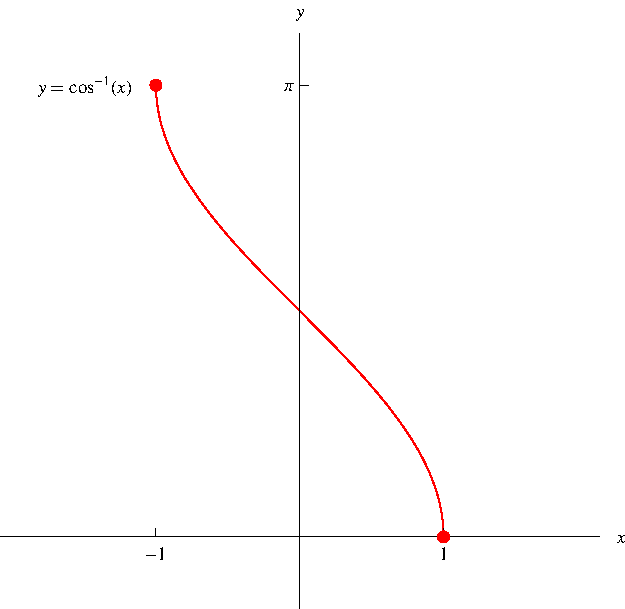
\includegraphics[height=6cm]{inverse-trig/pictures/07-06-arccosd.pdf}%
\column{.5\textwidth}
\begin{enumerate}
\item  \alert<handout:0| 2-3>{Domain: \uncover<3->{$[-1, 1]$.}}
\item  \alert<handout:0| 4-5>{Range: \uncover<5->{$[0, \pi ]$.}}
\item  $\cos^{-1} x = y \Leftrightarrow \cos y = x$ and $0 \leq y \leq \pi$.
\item  $\cos^{-1} (\cos x) = x$ for $0 \leq x \leq \pi$.
\item  $\cos (\cos^{-1} x) = x$ for $-1 \leq x \leq 1$.
\item  $\frac{\diff}{\diff x} (\cos^{-1} x) = -\frac{1}{\sqrt{1-x^2}}$.  \uncover<6->{(The proof is similar to the proof of the formula for the derivative of $\sin^{-1} x$.)}
\end{enumerate}
\end{columns}
\end{frame}
% end module arccos-properties

% begin module arctan-def
\begin{frame}
\begin{columns}[c]
\column{.5\textwidth}
\ \only<handout:0| -1>{%
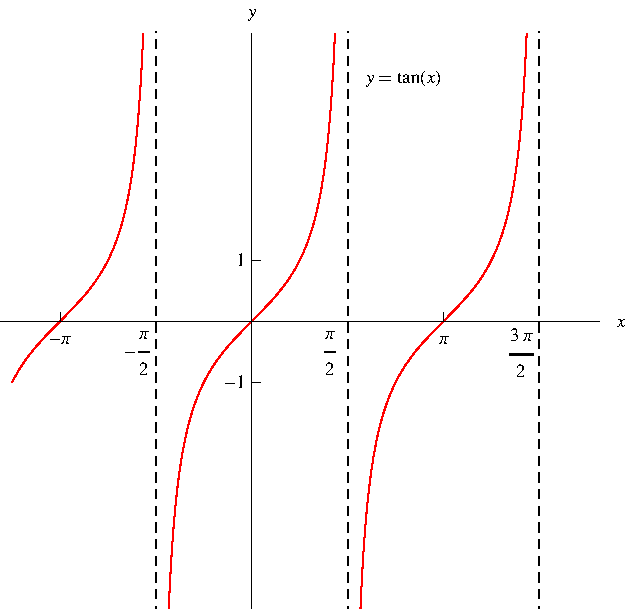
\includegraphics[width=5cm]{inverse-trig/pictures/07-06-arctana.pdf}%
}%
\only<handout:1| 2>{%
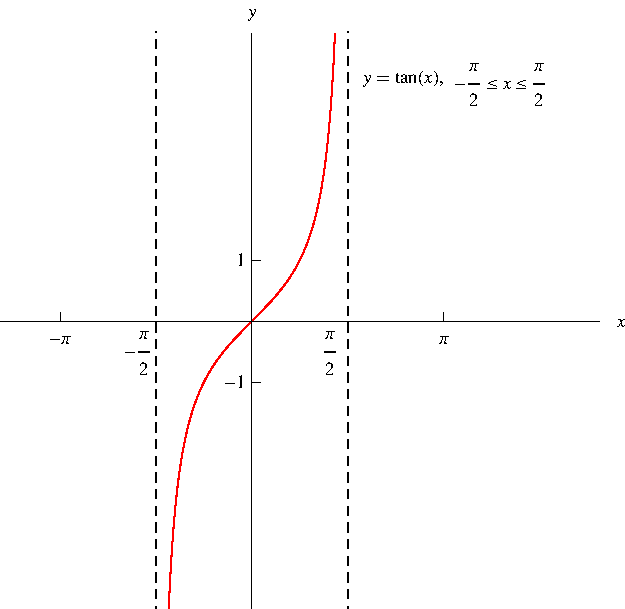
\includegraphics[width=5cm]{inverse-trig/pictures/07-06-arctanb.pdf}%
}%
\only<handout:2| 3->{%
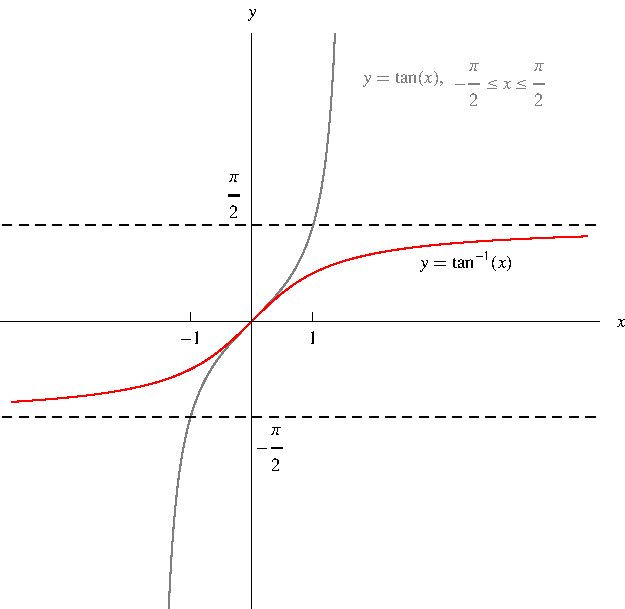
\includegraphics[width=5cm]{inverse-trig/pictures/07-06-arctanc.pdf}%
}%
\column{.5\textwidth}
\begin{itemize}
\item<1->  $\tan x$ isn't one-to-one.
\item<2->  Restrict the domain to $(-\pi /2, \pi /2)$.
\item<3->  The inverse is called $\Arctan$ or $\arctan$.
\item<4->  $\Arctan x = y \Leftrightarrow \tan y = x$ and $-\pi /2 < y < \pi /2$.
\item<5->  \alert<handout:0| 5-6>{Domain of $\Arctan$: \uncover<6-| handout:0>{$(-\infty,\infty)$.}}
\item<5->  \alert<handout:0| 7-8>{Range of $\Arctan$: \uncover<8-| handout:0>{$(-\pi / 2, \pi / 2)$.}}
\item<9->  \alert<handout:0| 9-10>{$\displaystyle \lim_{x\rightarrow \infty} \Arctan x = \uncover<10-| handout:0>{\pi / 2.}$}
\item<9->  \alert<handout:0| 11-12>{$\displaystyle \lim_{x\rightarrow - \infty} \Arctan x = \uncover<12-| handout:0>{- \pi / 2.}$}
\end{itemize}
\end{columns}
\end{frame}
% end module arctan-def



\end{document}
